







\newcommand{\robotimage}[1]{
\includegraphics[height=#1mm]{images/robot.png}}
\renewcommand{\notok}{
\includegraphics[height=5mm]{images/notok.png}}
\renewcommand{\ok}{
\includegraphics[height=5mm]{images/ok.png}}


%on veut des systèmes que l'on peut COMPRENDRE

%knowledge est important dès que plusieurs agents en interaction

% pas réaliste d'avoir que des systèmes centralisées

% 


%il y a toujours qqch de formel. Une image, une politique en reinforcement learning. Ici, on étudie des modèles.

\newcommand{\examplepreconditiondecision}[2]{\algoif #1 \algothen 
	
	~~~~~~~~ {\textcolor{gray}{\texttt{#2}}} 


~~

}

\begin{frame}
\frametitle{Reasoning about knowledge, useful in multi-agent systems}


\examplepreconditiondecision{\coloragenta{I know} it is safe}{I go}

%\examplepreconditiondecision{\coloragenta{I know} you are at the market place}{I join you}


\examplepreconditiondecision{(\coloragenta{I know} it is safe) and (\coloragenta{I know} \coloragentb{you do not know} it is safe)}{I tell you it is safe}


\examplepreconditiondecision{\coloragenta{I know} \coloragentb{you know} it is safe}{I do not tell you it is safe}




\examplepreconditiondecision{\coloragenta{I know} \coloragentb{you know} \coloragenta{I know} it is safe or not}{I do not wait for a message from you}


\pause

\begin{block}{}
	$\Rightarrow$ 
Dynamic epistemic logic to reason about knowledge.
\end{block}
\end{frame}




\begin{frame}
	\frametitle{Issue: logic can be very abstruse / boring}
	
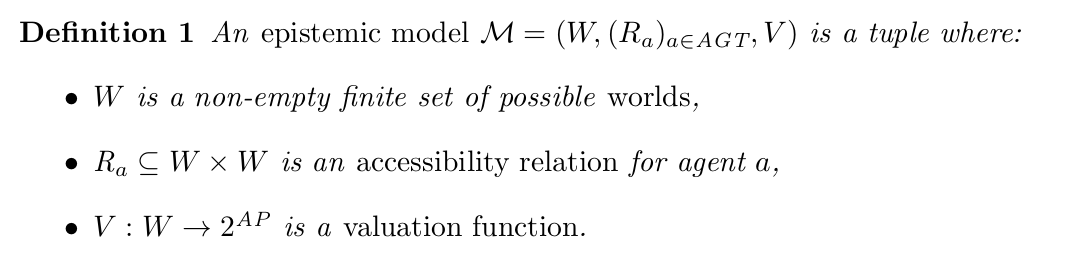
\includegraphics[width=\textwidth]{images/def_epistemic_model.png}
\end{frame}



\begin{frame}
	\frametitle{Solution: Hintikka's World}
	
	\begin{block}{}
Teach /	Explain Dynamic epistemic logic with comics!
	\end{block}
	
	\begin{center}
		
		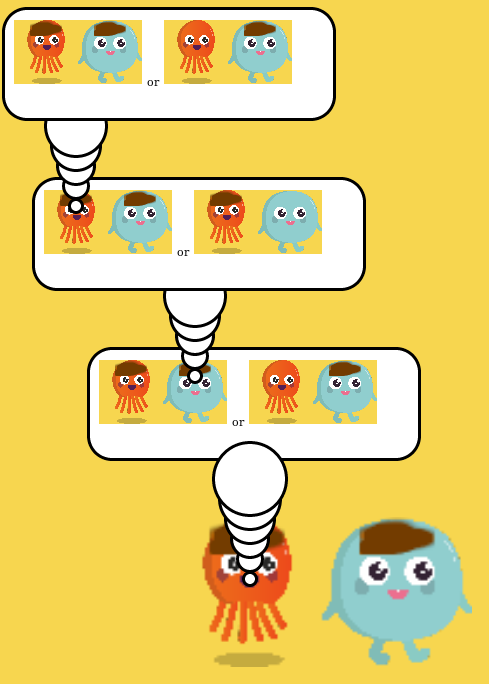
\includegraphics[width=3cm]{hintikka_world_screenshot.png}
		
		\url{http://hintikkasworld.irisa.fr/}
		
	
	\end{center}
\end{frame}


%The Knowledge of Preconditions Principle


